
\section{Non-inverting buck-boost converter\label{N_INV_BB}}
		
The Non-inverting Buck-Boost converter is a DC to DC converter that allows the voltage at its output to be higher or lower than the voltage at its input. The topology can be seen in figure \ref{N_INV_BB_SCHEMATIC}. It uses 4 switches, of which 2 are controlled devices. 
		

\begin{figure}[htbp]
	\begin{center}
	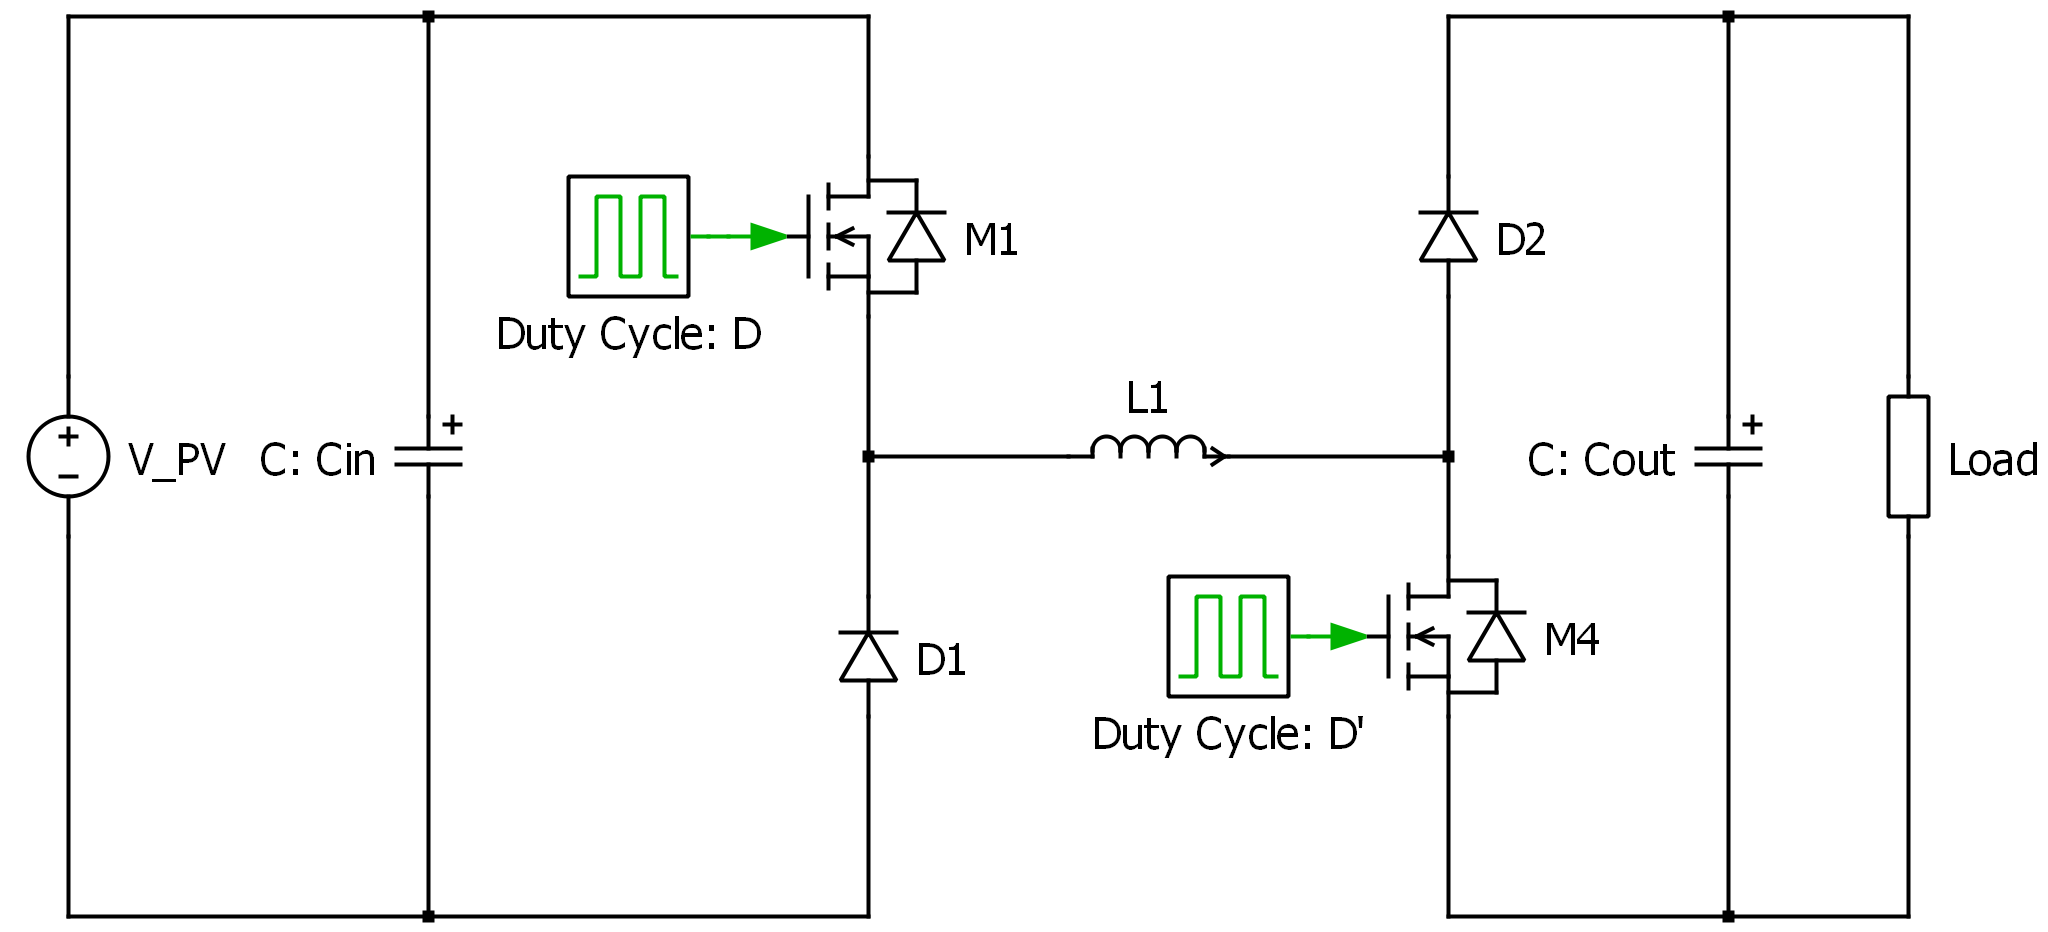
\includegraphics[width=0.7\textwidth]{../Pictures/2_d_H_B_BB}
	\caption{Non-inverting buck-boost converter.}
	\label{N_INV_BB_SCHEMATIC}
	\end{center}	
\end{figure}

		
The controller can force the system to work in any of the following modes:

\begin{enumerate}
	\item Buck $\rightarrow$ $ D \subset [0,1];	 D' = 0 $
	\item Boost $\rightarrow$ $ D = 1;	 D' \subset [0,1] $
	\item Buck-Boost $\rightarrow$ $ D \subset [0,1]; D' \subset [0,1] $
\end{enumerate}
		
Usually the inverter's input voltage is fixed to some value higher than the grid's voltage. The possibility of higher and lower voltages at the converter's output allows different ways of associating photovoltaic modules. Then the user is able to arbitrarily decide how many PV modules to link in series. Differently of what would happen in the case of Buck or Boost converters where the constraints regarding the number of panels are tighter.
		
Compared with other topologies that can have both higher and lower voltages at the output, such as the SEPIC converter, this DC-DC features a single inductor and no intermediate capacitor. See SEPIC schematic in figure \ref{SEPIC_SCHEMATIC}, notice the additional inductor and capacitor. With such reduction in passive components the price, efficiency and power density improves significantly \cite{underthehood}.

\begin{figure}[htbp]
	\begin{center}
		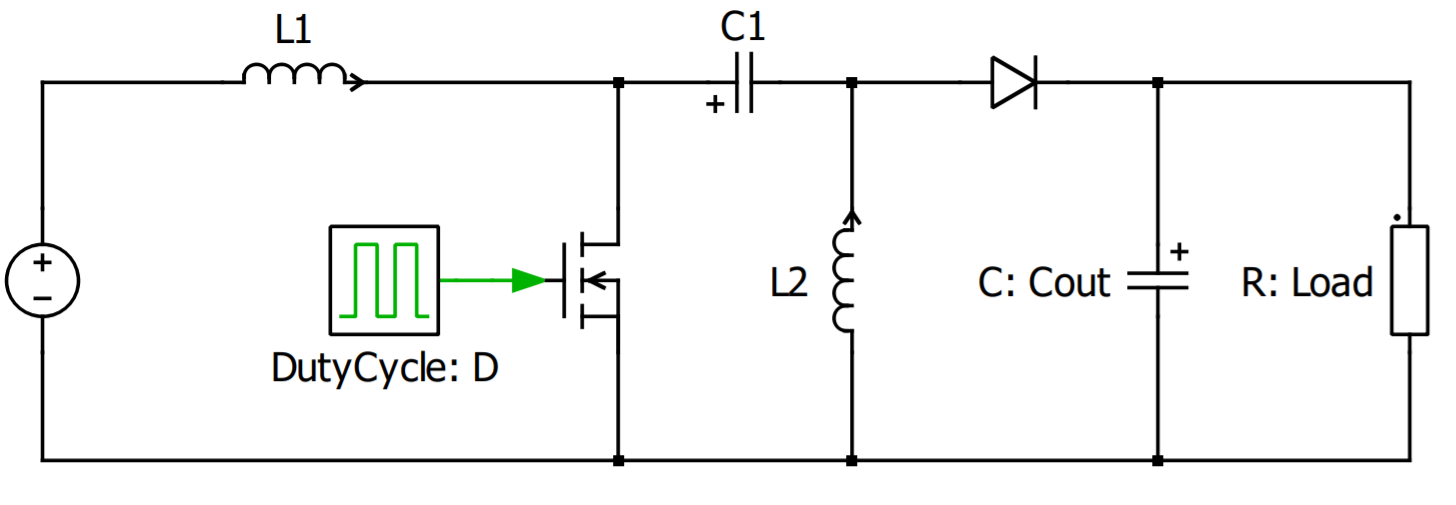
\includegraphics[width=0.7\textwidth]{../Pictures/SEPIC}
		\caption{SEPIC converter.}
		\label{SEPIC_SCHEMATIC}
	\end{center}	
\end{figure}

One of the main drawbacks of the non-inverting buck-boost topology is the control's complexity, which must calculate the appropriate duty cycle $D$ and $D'$ in any of the modes and also the transition between these modes. The buck-boost mode is specially complicated as there are two duty cycles to calculate. This problem might be addressed by setting a constant duty cycle in one of the bridge's legs and then the control will calculate the other leg's duty cycle  \cite{AN4449_ST}.
		
Although this topology exhibits appropriate features, it can be further improved by replacing the diodes by MOSFETs. The circuit may be seen in figure \ref{BID_N_INV_BB_SCHEMATIC}, it's called Bidirectional Non-Inverting Buck-Boost converter. With this variation, the following changes occur:
		
\begin{enumerate}
	\item The system becomes bidirectional.
	\item The conduction losses are smaller. 
\end{enumerate}
	
If the system is bidirectional it can be used in different MIC strategies, as the topology seen in figure \ref{BID_MIC_ARCHITECTURES}, which features an isolated dc link. This topology needs a bidirectional MIC as energy flow in both directions is needed. It also allows diagnosis of PV modules, as described in section \ref{selection_of_topology}.

\begin{figure}[htbp]
	\begin{center}
		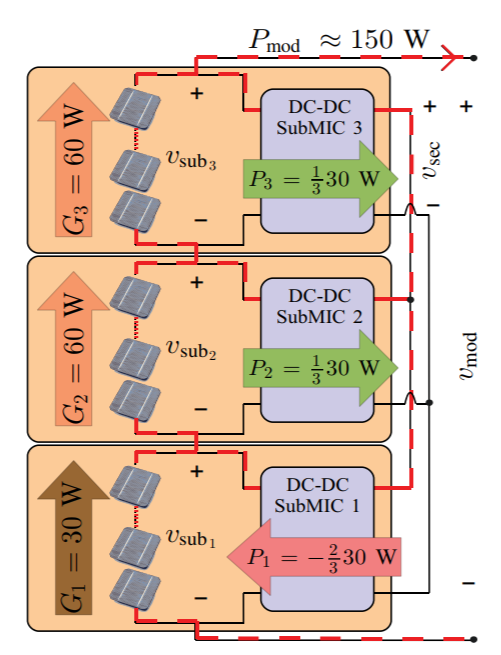
\includegraphics[width=0.4\textwidth]{../Pictures/bidirectional_mic_use}
		\caption{Bidirectional MIC use \cite{ArchitectureMIC}.}
		\label{BID_MIC_ARCHITECTURES}
	\end{center}	
\end{figure}
		
		
As seen in figure \ref{BID_N_INV_BB_SCHEMATIC}, notice that duty cycles of the switches that replace the diodes are $\overline{D}$ and $\overline{D'}$. This line over the variables means that it is the negated value of the original variable. The duty cycle is the boolean variable that indicates the conduction state of a switch. In the case of an enhancement switch, the switch is conducting whenever its driving duty cycle is equal to '1' and it is closed when its driving duty cycle is equal to '0'. 
		
The main drawback is the increased difficulty of the driver circuitry and the requirement of a dead time in order to avoid the short circuit of $FET_1$ and $FET_3$ or $FET_2$ and $FET_4$, which could damage the system. When using diodes, the system is intrinsically protected against a shoot-through event. 	
		
\begin{figure}[htbp]
	\begin{center}
	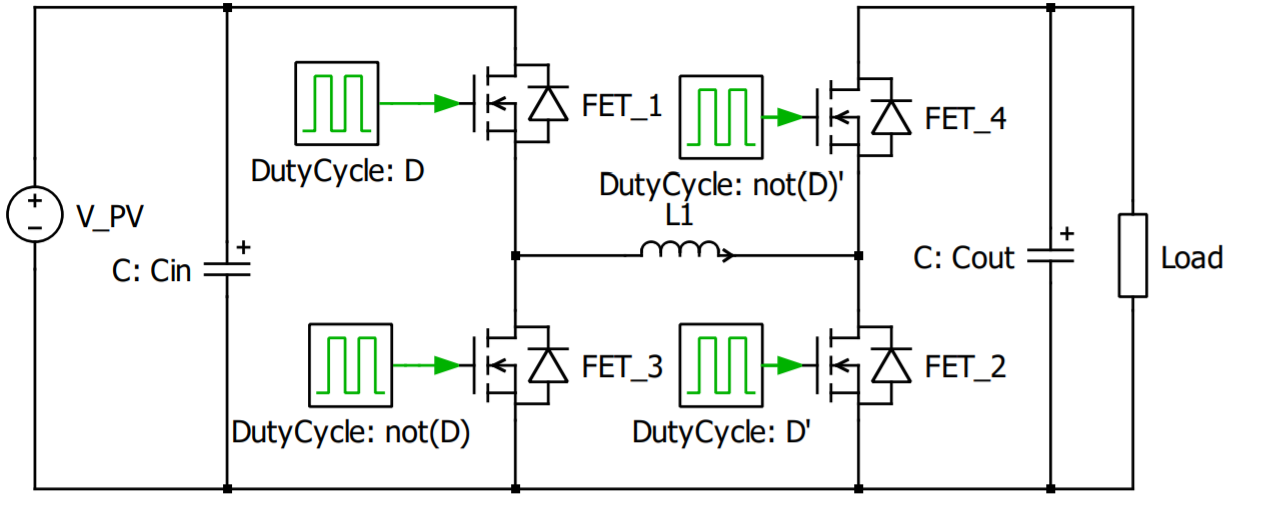
\includegraphics[width=0.7\textwidth]{../Pictures/BID_H_B_BB}
	\caption{Bidirectional Non-inverting buck-boost converter.}
	\label{BID_N_INV_BB_SCHEMATIC}
	\end{center}
\end{figure}



